\subsection {Simulation and analysis activities for the \MJ\ \MJDemo \label{MJDSimArticle}}

\auth{T.\,H.~Burritt,
\underline{M.~Buuck},
C.~Cuesta,
J.\,A.~Detwiler,
J.~Gruszko,
\underline{I.~Guinn},
D.\,A.~Peterson,
R.\,G.\,H.~Robertson,
and T.\,D.~Van Wechel
}

\noindent The UW \MJ\ group under the direction of Dr. Jason Detwiler leads the simulations and analysis effort within the \MJ\ collaboration. Much of the low-level software for data I/O, event building, data processing, and simulation were written by CENPA personnel. Members of our group have played a central role in the building and validation of the background model for the \MJ\ \MJDemo, which informs the radiopurity criteria upon which the experimental design is evaluated. We also participate in the development and implementation of data analysis techniques, geometrical models for Monte Carlo simulations, and data handling, storage, and database technologies. Our efforts over the past year have focused on workflow management, improvements to data processing and cleaning, and the development and use of analysis tools for data from the first commissioning run of the \MJ\ \MJDemo\ Module 1. A significant achievement for the collaboration this past year was the submission for publication of a paper on our muon veto system.

%As the Simulations and Analysis task leader for \MJ, Jason Detwiler oversees the development of the software tools necessary for full data taking. This past year, Detwiler implemented a working group structure to better organize the members of the collaboration around the software tasks at hand. This restructuring has been a great success, and has significantly accelerated the production of the \MJ\ software tools.
\begin{wrapfigure}{r}{0.5\textwidth}
\begin{center}
\hfil  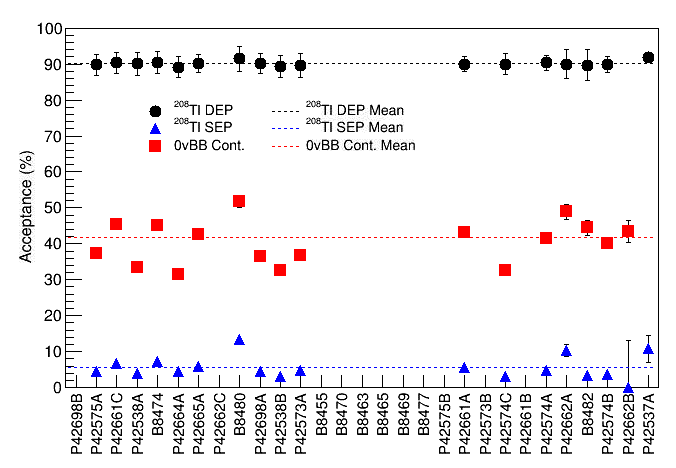
\includegraphics[width=.48\textwidth]{DS1_AoverECut_Efficiency_160330.png} \hfil 
% the following blank line is important

\end{center}
%Sorry Gary, but the default wasn't working with wrapfigure
\refstepcounter{figure} \hfil \parbox{.5\textwidth}{\small Figure~\ref{MJDSimArticle}-\arabic{figure}. A/E acceptances for all detectors in Module 1. The black circles show the acceptance in the \iso{208}{Tl} double-escape peak, which is dominated by single-site interactions. We tune the acceptance there to the expected fraction of \nonubb\ events that are single-site, which is 90\%. The technique is very successful at rejecting events in the \iso{208}{Tl} single-escape peak (blue triangles), which is dominated by multi-site interactions. The effect of the cut on backgrounds in the \iso{76}{Ge} \nonubb-decay region-of-interest is given for each detector by the red squares. }  \hfil

\label{AoE}  %put label{} after \figcaption{}

\end{wrapfigure}

In her role as head of the Data Cleaning and Run Selection working group, Dr. Clara Cuesta has continued to oversee the implementation and evaluation of the Data Cleaning and Run Selection framework for \MJ. Her work in this regard is detailed elsewhere \secref{}.\newline
\indent Dr. Cuesta has also led the development of a pulse-shape based background suppression technique called A/E which analyzes the ratio of the max current in a pulse to the energy collected. Events that produce a single localized energy deposit \--- such as most \nonubb\ decays \--- will have a larger value of A/E than events that deposit energy in multiple locations inside the same detector. We have shown using \iso{228}{Th} calibration data that we are able to reduce our backgrounds using this technique by more than 50\% (see \figref{MJDSimArticle}{AoE}).

Julieta Gruszko has collaborated in the development and largely herself implemented a new technique to tag events that occur near the passivated surface of the \MJ\ detectors. The technique compares the decay of waveforms after the rising edge, looking for differences in the effective decay constant. Preliminary results are presented elsewhere \secref{LAAttE}.
%These events, which could be due to degraded $\alpha$-particles, create some electron-hole pairs in the passivated layer. The holes are collected relatively quickly at the point-contact, but the electrons drift slowly out of the passivated layer, causing a small amount of delayed charge to be collected after the primary rising edge.

\begin{wrapfigure}{l}{0.5\textwidth}
\begin{center}
\hfil  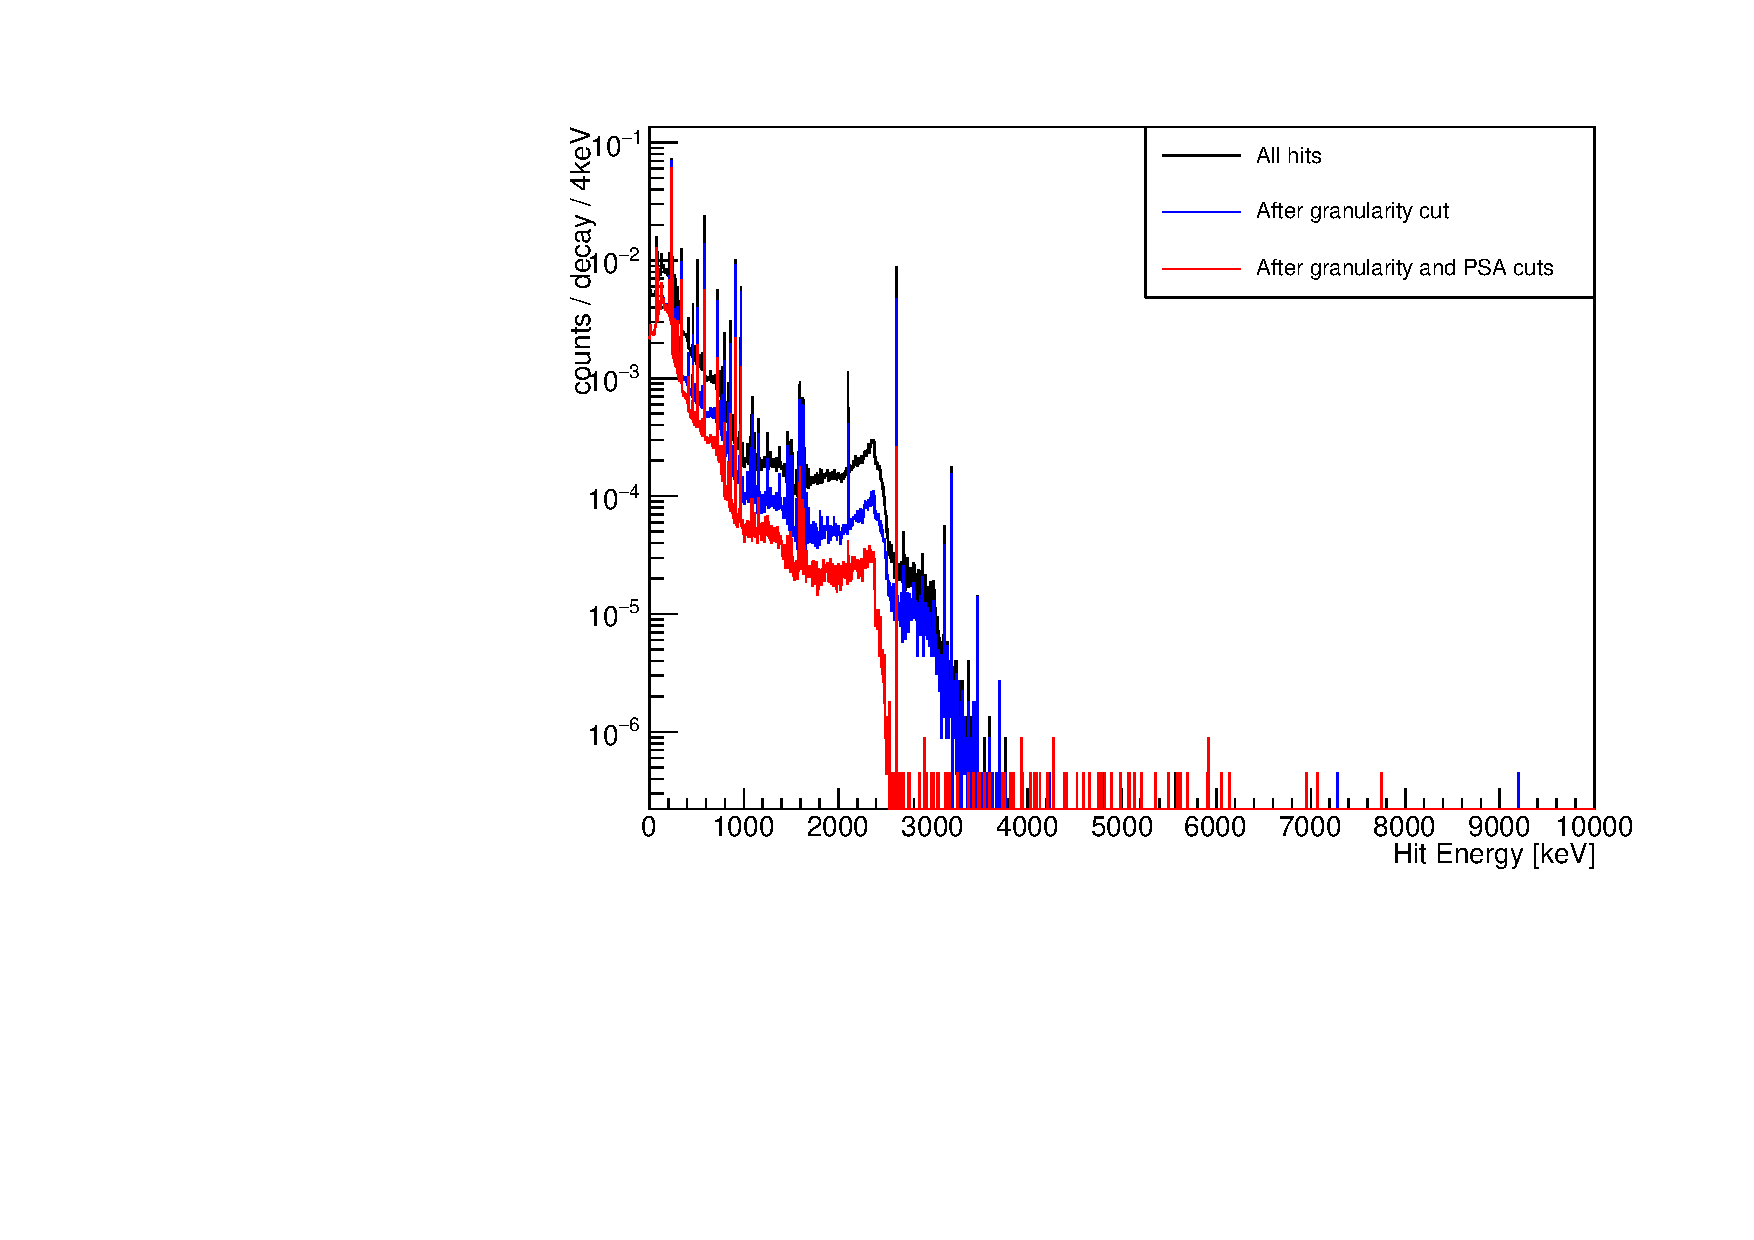
\includegraphics[width=.48\textwidth]{M1DUThCombined.pdf} \hfil 
% the following blank line is important

\end{center}
\refstepcounter{figure} \hfil \parbox{.5\textwidth}{\small Figure~\ref{MJDSimArticle}-\arabic{figure}. A simulation of the efficiency of the Module 1 array of Ge detectors for detecting thorium contamination in the copper detector unit pieces. The black line shows all energy depositions recorded by the array that do not occur in the dead layer of a detector. The blue line has removed events occurring in multiple detectors, and the red line has additionally removed events that are detectable as multi-site within a single detector. }  \hfil

\label{sim}  %put label{} after \figcaption{}

\end{wrapfigure}

Micah Buuck has primarily focused this year on two simulations- and analysis-related activities: a pulse-shape based technique for identifying multi-site backgrounds complementary to A/E, and upgrading the simulations software to produce results on the detector level.\newline
\indent The pulse-shape technique requires the generation of a ``basis library'' of single-site event pulses, which is then used to accept or reject incoming pulses based on a $\chi^2$ fit. He has successfully implemented the software necessary to generate the basis, and has done so on selected sets of calibration data. He is now in the process of quantifying the acceptance of the technique for various kinds of pulse shapes, and tuning input parameters to achieve optimal distinction between single- and multi-site pulses.\newline
\indent Buuck has also modified and upgraded the \MJ\ simulations post-processing software to incorporate detector-specific responses. He updated old code that determines which simulated interactions happen in the detector dead layers, and whether an event is likely to be distinguishable as multi-site. \figref{MJDSimArticle}{sim} is a simulation of the efficiency of the Module 1 array for detecting thorium contamination in the copper detector unit pieces. Each detector has a unique dead layer geometry and drift time mapping (primarily based on the detector shape) whose effects must be applied, before combining the data into a single spectrum. See the figure caption for description of the different lines.
%Micah Buuck has primarily been focused on implementing a pulse-shape-based analysis technique for rejection of background multi-site events. In this capacity, he is a part of the Pulse Shape working group. The technique requires the generation of a ``basis library'' of single-site event pulses, which is then used to accept or reject incoming pulses based on a $\chi^2$ fit. He has successfully implemented the software necessary to generate the basis, and is now working on streamlining the process and applying it to physics data.

Ian Guinn has continued to work on the event builder for the \MJ\ \MJDemo. The event builder has three main responsibilities. First, it converts the raw data files produced by the data acquisition system (ORCA) into ROOT files, known as built files, that are compatible with the \MJ\ software. Second, it combines waveforms and muon veto events that occur at nearby times into a single event, in order to detect coincidences. Finally, it filters out corrupted data that may confuse the main analysis software, a process known as garbage collection. In the last year, Guinn has implemented a builder for the muon veto data. He has also added a checker for built files, which searches for inconsistencies and errors that occur during the building process. Additionally, the event builder is now capable of building multi-sampled waveforms, in which the baseline and falling edge waveforms are sampled at a slower rate than the rising edge. Guinn has also made a number of other improvements and bug-fixes.\newline
\indent Guinn has also implemented a sophisticated algorithm for \MJ\ that fits peaks in the \MJDemo\ energy spectrum. The peak shape is composed of a gaussian, a high-energy exponential tail, a low-energy exponential tail, a flat background, and a step function. The peak fitter is used most importantly in calibrating the energy spectrum of the detectors. Guinn is currently working on extending the peak fitter to fit multiple peaks simultaneously, which will allow for faster and more robust energy calibration. Perhaps insert peakfitter image here?
%Julieta Gruszko has successfully implemented and begun to use new frequency-domain analysis techniques. She will use the techniques to identify and eliminate noise sources and for data cleaning. The resulting noise curves of detector baselines will be used to characterize the detector, to accurately simulate pulses, and for optimum filtering. The tools she developed this year allow researchers to view noise curves over time, which can be used to identify intermittent noise sources and therefore tag events for data cleaning. Average noise curves taken with the Prototype Cryostat system are being used to identify the optimal electronics setup and laboratory conditions for data taking. For an example, see \figref{MJDSimArticle}{Fluorescent_Lights}.
%
%
%\begin{figure}[h]
%\begin{minipage}{.5\textwidth}
%
%\hfil  \includegraphics[width=\textwidth]{MJFluorLights.jpeg} \hfil 
%% the following blank line is important
%
%\figcaption{MJDSimArticle}{A comparison of the white noise levels showed that the use of fluorescent lights in the lab was introducing noise. Following this study, the shielding of module electronics box was improved.}
%
%\label{Fluorescent_Lights}  %put label{} after \figcaption{}
%
%\end{minipage}
%\begin{minipage}{.5\textwidth}
%
%\hfil \includegraphics[width=\textwidth]{MJBGSpectrum.pdf} \hfil
%
%\figcaption{MJDSimArticle}{Full-spectrum background model for the MAJORANA DEMONSTRATOR, with and without analysis cuts.}
%
%\label{MJBGSpectrum}
%
%\end{minipage}
%\end{figure}
%

We are now analyzing the first data to come from the first module of enriched Ge detectors, and have recently commenced blind data taking. Other major activities include software quality assurance tests, utilization of run and detector information stored in our databases, automatic data workflow management, refinement of event building routines, optimization of energy estimation and pulse-shape parameter extraction algorithms, and data monitoring and cleaning routines.
%New assay results have improved the predicted background rate in the 4-keV region of interest surrounding the 2039 keV Q-value for double-beta decay of ${}^{76}$Ge to 3.1 counts/ton-year. Major simulation campaigns are underway to provide up-to-date predictions for the full spectrum we expect to see with enriched detector data. \figref{MJDSimArticle}{MJBGSpectrum} shows the full simulated spectrum, including the effect of analysis cuts. Other major activities include software quality assurance tests, database implementation of run information recording and automatic data workflow management, refinement of event building routines, optimization of energy estimation and pulse-shape parameter extraction algorithms, and data monitoring and cleaning routines.
